% ============================================================================
% IGVC 2026 Design Report --- Mechanical Section
% Cal Poly Pomona Autonomous Vehicle Lab
% Standalone subteam document; section numbering starts at 4 to match the
% report-level layout (1.Team / 2.Architecture / 3.Innovations / 4.Mechanical).
% ============================================================================
\documentclass[11pt, letterpaper]{article}

\usepackage[margin=1in]{geometry}
\usepackage{graphicx}
\usepackage{booktabs}
\usepackage{tabularx}
\usepackage{amsmath}
\usepackage{amssymb}
\usepackage{hyperref}
\usepackage{xcolor}
\usepackage{float}
\usepackage{enumitem}
\usepackage{caption}
\usepackage{subcaption}
\usepackage{tikz}
\usepackage{fancyhdr}
\usepackage{titlesec}
\usepackage{array}
\usepackage{multirow}
\usepackage[T1]{fontenc}

\usetikzlibrary{shapes.geometric, shapes.misc, arrows.meta, positioning, fit, calc, backgrounds, decorations.pathreplacing, patterns}

% ---- Colors (match report-level palette) ----
\definecolor{cppgreen}{RGB}{30, 90, 50}
\definecolor{codeblue}{RGB}{0, 80, 160}
\definecolor{warnred}{RGB}{180, 40, 40}
\definecolor{lightgray}{RGB}{230, 230, 230}

\hypersetup{colorlinks=true, linkcolor=cppgreen, citecolor=cppgreen, urlcolor=codeblue}

% ---- Headers / Footers ----
\pagestyle{fancy}
\fancyhf{}
\fancyhead[L]{\small Cal Poly Pomona Autonomous Vehicle Lab}
\fancyhead[R]{\small IGVC 2026 --- Mechanical}
\fancyfoot[C]{\thepage}
\renewcommand{\headrulewidth}{0.4pt}

% ---- Section formatting (match autonomy) ----
\titleformat{\section}{\large\bfseries\color{cppgreen}}{\thesection.}{0.5em}{}
\titleformat{\subsection}{\normalsize\bfseries}{\thesubsection}{0.5em}{}
\titlespacing*{\section}{0pt}{1.2ex}{0.6ex}
\titlespacing*{\subsection}{0pt}{0.8ex}{0.3ex}

% ---- Macros ----
\newcommand{\placeholder}[1]{\textcolor{warnred}{\textbf{[#1]}}}
\newcommand{\robotname}{PLACEHOLDER\_ROBOT\_NAME}

% Tighter lists
\setlist[itemize]{noitemsep, topsep=2pt, leftmargin=*}
\setlist[enumerate]{noitemsep, topsep=2pt, leftmargin=*}

% Start at section 4 so this standalone PDF matches the report layout.
\setcounter{section}{3}

\captionsetup{font=small, labelfont={bf,color=cppgreen}}

\begin{document}

% ============================================================================
% 4. MECHANICAL DESIGN
% ============================================================================
\section{Mechanical Design}

\subsection{Overview}

As first-year IGVC participants, the mechanical subteam prioritized a simple, modular,
and cost-effective platform that concentrates budget on the sensors and compute
required for autonomous navigation. \robotname{} is built on the commercially available
AndyMark\textsuperscript{\textregistered} Raptor Track Drive, a tracked differential
base selected for its all-terrain traction and short delivery lead time. A reconfigurable
80/20 T-slot aluminum superstructure is mounted directly to the chassis, allowing rapid
iteration on sensor mounts and shelf geometry through the design cycle. The same chassis
can host different electronics housings for future competitions; for IGVC~2026 the
housing is mounted on the upper shelf so that the electronics, payload, and E-stop are
all readily accessible during operation and inspection. Figure~\ref{fig:cad_iso} shows
the integrated vehicle.

\begin{figure}[H]
    \centering
    \begin{subfigure}[t]{0.48\linewidth}
        \centering
        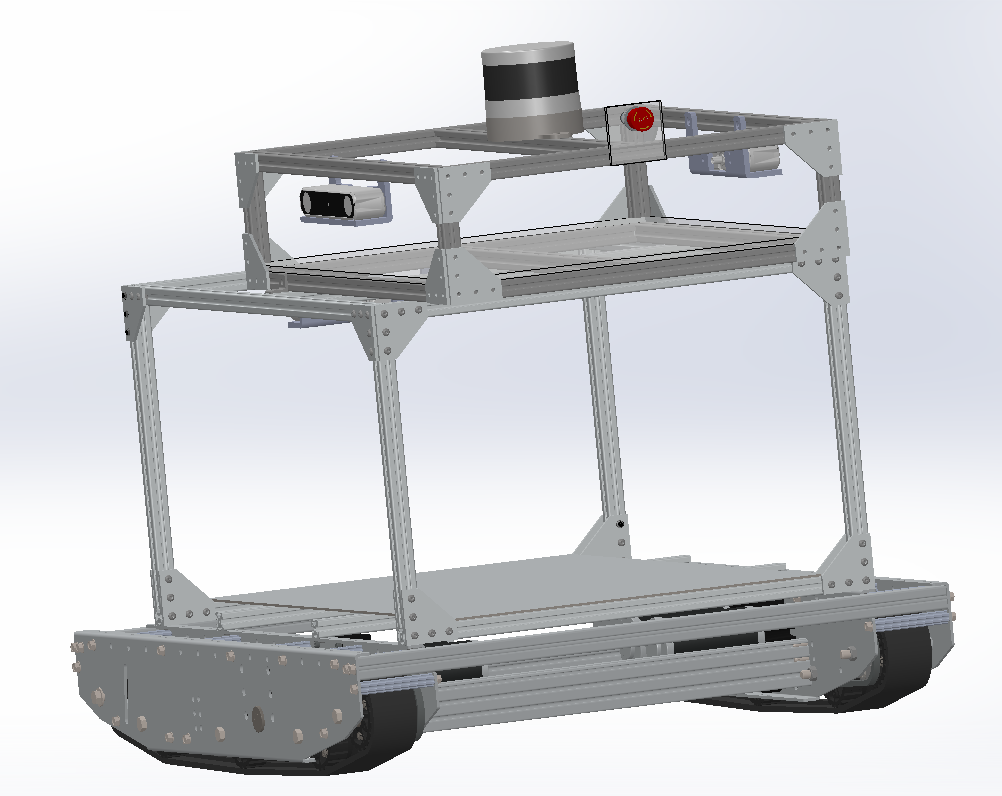
\includegraphics[width=\linewidth, trim=10 10 10 10, clip]{figures/cad_isometric.png}
        \caption{Front-quarter view showing the elevated sensor shelf, payload bay, and tracked base.}
        \label{fig:cad_iso}
    \end{subfigure}\hfill
    \begin{subfigure}[t]{0.48\linewidth}
        \centering
        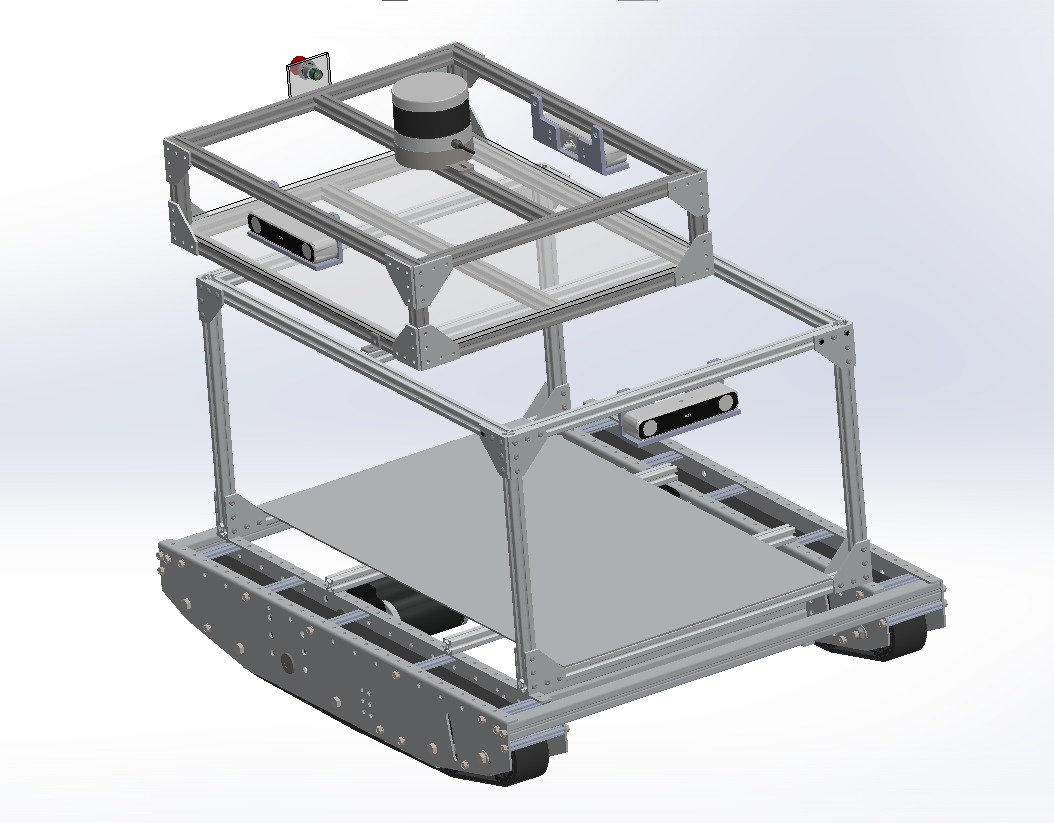
\includegraphics[width=\linewidth, trim=10 10 10 10, clip]{figures/cad_rear.png}
        \caption{Rear three-quarter view; rear-mounted shelf supports the mechanical E-stop and extends the chassis to meet the 3~ft length minimum.}
        \label{fig:cad_rear}
    \end{subfigure}
    \caption{CAD renders of \robotname{}: AndyMark Raptor base with 80/20 T-slot superstructure, diamond-plate payload deck, and 20~in elevated sensor shelf.}
    \label{fig:cad_overview}
\end{figure}

\subsection{Frame Structure and Chassis Integration}

The Raptor base contributes the drive sprockets, idlers, and rubber-track belts that
distribute vehicle weight over a large contact patch, improving traction and stability
on the uneven turf and gravel sections of the IGVC course. A $21.5~\text{in} \times 30~\text{in}$,
$1/8$~in thick A36 diamond-plate steel base is bolted directly to the Raptor mounting
rails. The diamond plate serves three functions: (i) a rigid surface for heavy
components, (ii) an EMI-attenuating ground plane between battery and tracked drive, and
(iii) a low-mounted mass that lowers the center of gravity.

The superstructure is built from 80/20\textsuperscript{\textregistered} 20-Series T-slot
aluminum extrusion. T-slot construction is modular and reconfigurable, eliminates exposed
threaded ends (T-slot nuts ride inside the channel), and lets the team prototype new
sensor mounts in minutes with 3D-printed brackets. The sensor shelf, payload mount, and
acrylic weather panels all attach to the same 20-Series profile.

Weight placement was an explicit design priority. The 48~V battery pack --- the heaviest
single component on the vehicle --- is mounted at the geometric \textit{center} of the
diamond plate so that its mass contributes minimally to pitch and yaw inertia. The 20~lb
payload bay sits at the \textit{front} of the deck on a 3D-printed cradle so it remains
accessible for inspection and so the operator can verify payload retention from outside
the chassis. The resulting load distribution (Figure~\ref{fig:weight_dist}) places the
center of gravity slightly forward of the track midpoint, biased toward the payload
end; because both heavy masses sit low on the diamond-plate deck, the overall CoG height
is minimized and the vehicle remains stable on inclines and during skid-steer turns.
Table~\ref{tab:specs} summarizes the resulting vehicle parameters.

% ----- Weight distribution figure (Phase 3 will replace placeholder) -----
\begin{figure}[H]
    \centering
    % Side view of the vehicle showing payload (front) and battery (centered) on the
% diamond-plate deck, with center-of-gravity marker biased forward of the track
% midpoint. Muted palette; safety-red reserved for the E-stop and CoG marker only.
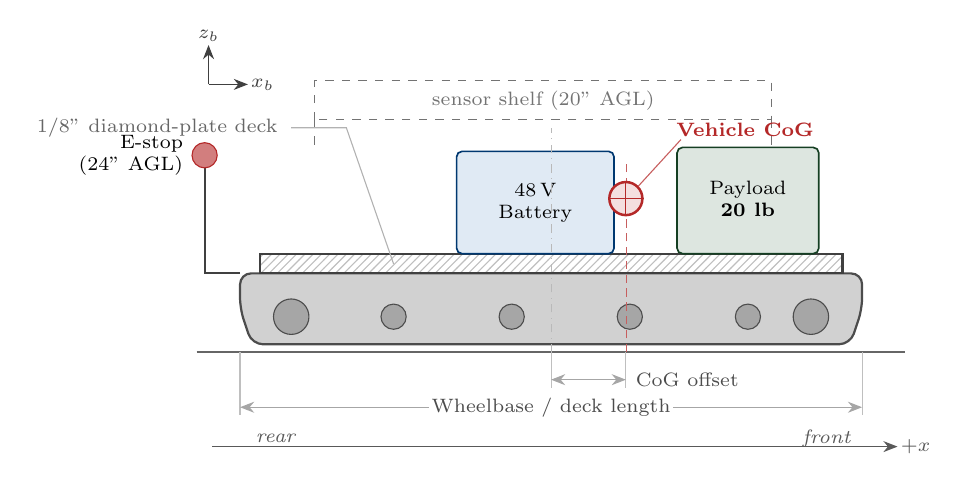
\begin{tikzpicture}[
    font=\footnotesize,
    >={Stealth[length=1.8mm, width=1.4mm]},
    obj/.style={draw, thick, black!75},
    track/.style={draw=black!70, thick, fill=black!18, rounded corners=4pt},
    wheel/.style={draw=black!70, circle, fill=black!35, minimum size=0.45cm, inner sep=0pt},
    deck/.style={draw=black!75, thick, fill=black!8, pattern=north east lines, pattern color=black!25},
    payload/.style={draw=cppgreen!70!black, semithick, fill=cppgreen!15, rounded corners=2pt},
    battery/.style={draw=codeblue!70!black, semithick, fill=codeblue!12, rounded corners=2pt},
    shelf/.style={draw=black!55, thin, dashed, fill=none},
    dim/.style={<->, gray!70, thin},
    extline/.style={gray!50, thin},
    dimtxt/.style={font=\scriptsize, gray!60!black},
    cogmark/.style={circle, draw=warnred, line width=0.9pt, fill=warnred!15, minimum size=0.42cm, inner sep=0pt},
    refline/.style={gray!55, very thin, dash dot},
    cogline/.style={warnred!75, very thin, densely dashed},
]

% --- Ground line (clean baseline, no hatched ticks competing for ink) ---
\draw[black!60, semithick] (-0.5, 0) -- (8.5, 0);

% --- Track outline (side view): rounded rectangle, wheels visible ---
\draw[track] (0.2,0.1) -- (7.8,0.1) -- (7.95,0.55) -- (7.95,1.0) -- (0.05,1.0) -- (0.05,0.55) -- cycle;
\node[wheel] at (0.7, 0.45) {};
\node[wheel] at (7.3, 0.45) {};
\foreach \x in {2.0,3.5,5.0,6.5}{ \node[wheel, minimum size=0.32cm] at (\x, 0.45) {}; }

% --- Diamond plate deck on top of tracks ---
\draw[deck] (0.3, 1.0) rectangle (7.7, 1.25);
\node[dimtxt, anchor=south, font=\scriptsize\itshape] at (4.0, 1.28) {\hspace*{4cm}}; % placeholder kept blank — deck label moved below

% --- Sensor shelf (downplayed: dashed outline only, no fill) ---
\draw[shelf] (1.0, 2.95) rectangle (6.8, 3.45);
\node[font=\scriptsize, black!55] at (3.9, 3.20) {sensor shelf (20'' AGL)};
\draw[shelf, thin] (1.0, 2.95) -- (1.0, 2.6);  % shelf supports
\draw[shelf, thin] (6.8, 2.95) -- (6.8, 2.6);

% --- Payload (front = right) ---
\draw[payload] (5.6, 1.25) rectangle (7.4, 2.6);
\node[align=center, font=\scriptsize] at (6.5, 1.95) {Payload\\\textbf{20 lb}};

% --- Battery (centered on deck) ---
\draw[battery] (2.8, 1.25) rectangle (4.8, 2.55);
\node[align=center, font=\scriptsize] at (3.8, 1.9) {48\,V\\Battery};

% --- Rear E-stop standoff (red reserved for safety) ---
\draw[obj] (0.05, 1.0) -- (-0.4, 1.0) -- (-0.4, 2.4);
\node[draw=warnred, circle, fill=warnred!60, minimum size=0.32cm, inner sep=0pt] at (-0.4, 2.5) {};
\node[font=\scriptsize, anchor=east, align=right] at (-0.55, 2.5) {E-stop\\(24'' AGL)};

% --- Reference centerlines: track midpoint (gray) and CoG drop (red) ---
\draw[refline] (4.0, 0) -- (4.0, 2.85);
\draw[cogline] (4.95, 0) -- (4.95, 2.40);

% --- CoG marker (placed in gap between battery and payload, large + ringed) ---
\node[cogmark] (cog) at (4.95, 1.95) {};
\draw[warnred, thin] (cog.north) -- (cog.south);
\draw[warnred, thin] (cog.east)  -- (cog.west);
% Leader from label to marker; explicit "Vehicle CoG" so it's not confused with payload's own CoG
\draw[warnred!75, thin] (5.65, 2.70) -- (cog.north east);
\node[font=\scriptsize\bfseries, warnred, anchor=south west, inner sep=1pt] at (5.55, 2.70) {Vehicle CoG};

% --- Body-frame coordinate marker (top-left of plot) ---
\begin{scope}[shift={(-0.35, 3.4)}]
    \draw[->, black!75, thin] (0,0) -- (0.5,0) node[font=\scriptsize, anchor=west, inner sep=1pt]{$x_b$};
    \draw[->, black!75, thin] (0,0) -- (0,0.5) node[font=\scriptsize, anchor=south, inner sep=1pt]{$z_b$};
\end{scope}

% --- Dimension strip well below the chassis (clean margin) ---
\draw[extline] (0.05, 0)    -- (0.05, -0.80);
\draw[extline] (7.95, 0)    -- (7.95, -0.80);
\draw[extline] (4.0, 0)     -- (4.0, -0.45);
\draw[extline] (4.95, 0)    -- (4.95, -0.45);
\draw[dim] (4.0, -0.35) -- (4.95, -0.35);
\node[dimtxt, anchor=west, inner sep=2pt] at (5.0, -0.35) {CoG offset};
\draw[dim] (0.05, -0.70) -- (7.95, -0.70);
\node[dimtxt, fill=white, inner sep=1pt] at (4.0, -0.70) {Wheelbase / deck length};

% --- Front / rear axis at the very bottom ---
\node[font=\scriptsize\itshape, gray!70!black] at (0.5, -1.10) {rear};
\node[font=\scriptsize\itshape, gray!70!black] at (7.5, -1.10) {front};
\draw[->, gray!70!black, thin] (-0.3,-1.20) -- (8.4,-1.20) node[font=\scriptsize, anchor=west, inner sep=1pt]{$+x$};

% --- Deck material leader (callout from above the deck) ---
\draw[gray!60, thin] (2.0, 1.12) -- (1.4, 2.85) -- (0.7, 2.85);
\node[font=\scriptsize, black!60, anchor=east] at (0.65, 2.85) {1/8'' diamond-plate deck};

\end{tikzpicture}

    \caption{Side-view weight distribution. The 48~V battery is mounted at the geometric
    center of the diamond-plate deck and the 20~lb payload sits at the front. With the
    payload biasing the load forward of the heavy battery, the center of gravity (CoG)
    sits slightly forward of the track midpoint. Placing both heavy masses low on the
    deck minimizes overall CoG height and reduces pitch moment during braking and
    sloped traversal.}
    \label{fig:weight_dist}
\end{figure}

% ----- Frame top-view with dimensions -----
\begin{figure}[H]
    \centering
    % Top-down dimensioned view of the chassis: tracks on the sides, diamond-plate
% deck inside, sensor shelf outline (dashed) above. Dimensions show the deck
% size (21.5x30), shelf size (23x23), and overall length.
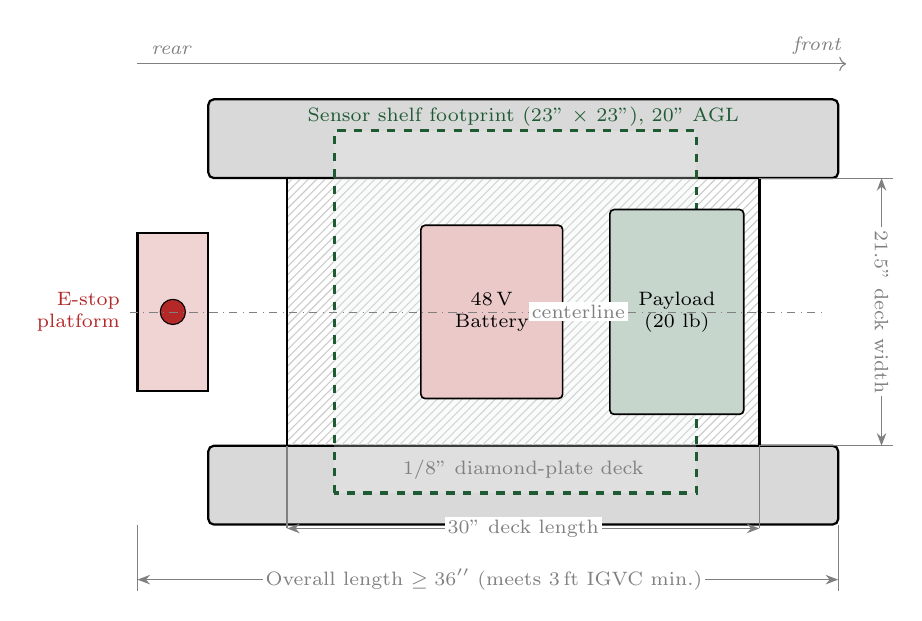
\begin{tikzpicture}[
    font=\footnotesize,
    track/.style={draw, thick, fill=gray!30, rounded corners=2pt},
    deck/.style={draw, thick, fill=gray!10, pattern=north east lines, pattern color=gray!40},
    shelf/.style={draw, very thick, dashed, cppgreen, fill=cppgreen!8, fill opacity=0.25, text opacity=1.0},
    payload/.style={draw, semithick, fill=cppgreen!25, rounded corners=1.5pt},
    battery/.style={draw, semithick, fill=warnred!25, rounded corners=1.5pt},
    dim/.style={<->, >={Stealth[length=1.6mm]}, gray, semithick},
    extline/.style={gray, thin},
    dimtxt/.style={font=\scriptsize, gray, fill=white, inner sep=1pt},
]

% --- Tracks (top view: two long rectangles) ---
\draw[track] (0,0) rectangle (8.0, 1.0);    % bottom track strip
\draw[track] (0,4.4) rectangle (8.0, 5.4);  % top track strip

% --- Diamond plate deck between the tracks ---
\draw[deck] (1.0, 1.0) rectangle (7.0, 4.4);

% --- Sensor shelf outline (projected) — DRAWN BEFORE PAYLOAD/BATTERY ---
% Translucent so the items beneath remain visible
\draw[shelf] (1.6, 0.4) rectangle (6.2, 5.0);

% --- Battery (centered on deck) and payload (front, RIGHT) ---
\draw[battery] (2.7, 1.6) rectangle (4.5, 3.8);
\node[align=center, font=\scriptsize] at (3.6, 2.7) {48\,V\\Battery};

\draw[payload] (5.1, 1.4) rectangle (6.8, 4.0);
\node[align=center, font=\scriptsize] at (5.95, 2.7) {Payload\\(20 lb)};

% --- Deck label below the deck (not floating inside) ---
\node[font=\scriptsize, gray, anchor=north] at (4.0, 0.95) {1/8'' diamond-plate deck};

% --- Sensor shelf labels: keep above the figure, away from inner content ---
\node[cppgreen, font=\scriptsize] at (4.0, 5.18) {Sensor shelf footprint (23'' $\times$ 23''), 20'' AGL};

% --- Rear E-stop platform extension ---
\draw[thick, fill=warnred!20] (-0.9, 1.7) rectangle (0.0, 3.7);
\node[draw, circle, fill=warnred, minimum size=0.32cm, inner sep=0pt] at (-0.45, 2.7) {};
\node[font=\scriptsize, anchor=east, warnred, align=right] at (-1.0, 2.7) {E-stop\\platform};

% --- Front / rear flow arrow (placed above the upper track to avoid overlap) ---
\draw[->, gray] (-0.9, 5.85) -- (8.1, 5.85);
\node[font=\scriptsize\itshape, gray, anchor=south east] at (-0.1, 5.85) {rear};
\node[font=\scriptsize\itshape, gray, anchor=south west] at (7.3, 5.85) {front};

% --- Dimension: deck length (30 in) ---
\draw[extline] (1.0, 1.0) -- (1.0, -0.05);
\draw[extline] (7.0, 1.0) -- (7.0, -0.05);
\draw[dim] (1.0, -0.05) -- (7.0, -0.05);
\node[dimtxt] at (4.0, -0.05) {30'' deck length};

% --- Dimension: deck width (21.5 in) vertical, right side ---
\draw[extline] (7.0, 1.0) -- (8.7, 1.0);
\draw[extline] (7.0, 4.4) -- (8.7, 4.4);
\draw[dim] (8.55, 1.0) -- (8.55, 4.4);
\node[dimtxt, rotate=-90] at (8.55, 2.7) {21.5'' deck width};

% --- Dimension: overall length incl. E-stop platform ---
\draw[extline] (-0.9, 0.0) -- (-0.9, -0.85);
\draw[extline] (8.0, 0.0) -- (8.0, -0.85);
\draw[dim] (-0.9, -0.7) -- (8.0, -0.7);
\node[dimtxt] at (3.5, -0.7) {Overall length $\geq 36''$ (meets 3\,ft IGVC min.)};

% --- Centerline (faint, broken at center to not collide with width label) ---
\draw[gray, very thin, dash dot] (-1.0, 2.7) -- (7.8, 2.7);
\node[font=\scriptsize, gray, anchor=center, fill=white, inner sep=1pt] at (4.7, 2.7) {centerline};

\end{tikzpicture}

    \caption{Top-view footprint and key dimensions. The diamond-plate deck
    ($21.5'' \times 30''$) hosts battery and payload; the upper sensor shelf
    ($23'' \times 23'' \times 6''$) sits 20~in above ground, providing a $24''$
    e-stop mounting height (rear shelf) and clear lines of sight for LiDAR and cameras.}
    \label{fig:frame_dims}
\end{figure}

\begin{table}[H]
    \centering
    \small
    \caption{\robotname{} vehicle specifications.}
    \label{tab:specs}
    \begin{tabular}{l l}
        \toprule
        \textbf{Parameter} & \textbf{Value} \\
        \midrule
        Drive configuration & Tracked differential (skid-steer) \\
        Base platform & AndyMark Raptor Track Drive \\
        Overall length $\times$ width & $\sim 36'' \times 24''$ (meets 3~ft min.) \\
        Sensor-shelf height & $20''$ (top surface) \\
        E-stop mounting height & $24''$ (rear shelf, centered) \\
        Payload capacity (verified) & $\geq 20$~lb \\
        Drive motors & 2$\times$ REV NEO brushless (12--48~V) \\
        Motor controllers & 2$\times$ REV SparkMAX (CAN, 1~Mbit/s) \\
        Battery pack & 48~V lithium, rear-mounted \\
        Frame material & 80/20 20-Series T-slot aluminum extrusion \\
        Deck material & 1/8'' A36 diamond-plate steel \\
        Weather panels & Polycarbonate / acrylic in T-slot grooves \\
        \bottomrule
    \end{tabular}
\end{table}

\subsection{Drive System}

\robotname{} uses a tracked \textbf{differential-drive} architecture: two REV NEO
brushless motors, each commanded by a REV SparkMAX controller over CAN, independently
drive the left and right track loops. The choice eliminates steering linkages, reduces
the part count, and produces a control plant that maps cleanly onto the ROS~2 Nav2 / MPPI
controller running on the Jetson. With $v_L$ and $v_R$ the left and right track linear
velocities, the body-frame linear and angular rates are
\begin{align}
    v &= \tfrac{1}{2}(v_R + v_L), &
    \omega &= \tfrac{1}{b}(v_R - v_L),
\end{align}
where $b$ is the track width (effective lever arm between contact patches). The three
operating modes used by the planner are illustrated in
Figure~\ref{fig:diff_drive_kinematics}.

\begin{itemize}
    \item \textbf{Pivot turn:} one track is held stationary while the other drives forward
    ($v_L=0$, $v_R>0$, or vice versa). The robot rotates about the stationary contact
    patch with radius $r = b/2$.
    \item \textbf{In-place rotation (spin):} the tracks rotate in opposite directions at
    equal magnitude ($v_R = -v_L$). The instantaneous center of rotation (ICR) lies on
    the geometric center, yielding zero translation and maximum yaw rate. This mode is
    essential for the tight sequential-cone obstacle sections of the AutoNav course.
    \item \textbf{Gradual curve:} both tracks move forward with $v_R \neq v_L$. The ICR
    lies outside the contact patch and the turning radius is $R = \tfrac{b}{2}\,
    \tfrac{v_R + v_L}{v_R - v_L}$.
\end{itemize}

\begin{figure}[H]
    \centering
    % Differential-drive kinematics: pivot / in-place spin / gradual curve.
% Three panels share a single drawing convention so panels can be compared.
%
% Conventions:
%   - Top view, vehicle nose pointing UP (+x_b is forward)
%   - Each track's linear velocity is drawn as a blue arrow whose length
%     is proportional to |v|, with a reference length of REFVEL cm for |v|=v
%   - ICR is a red ringed dot; the upright acronym "ICR" is set with
%     \mathrm{} so it matches the typographic family of v_L, v_R, b
%   - Track width b is dimensioned in panel (a); the same b applies to (b),(c)
%   - Body-frame axes (x_b, y_b) appear once, in panel (b)
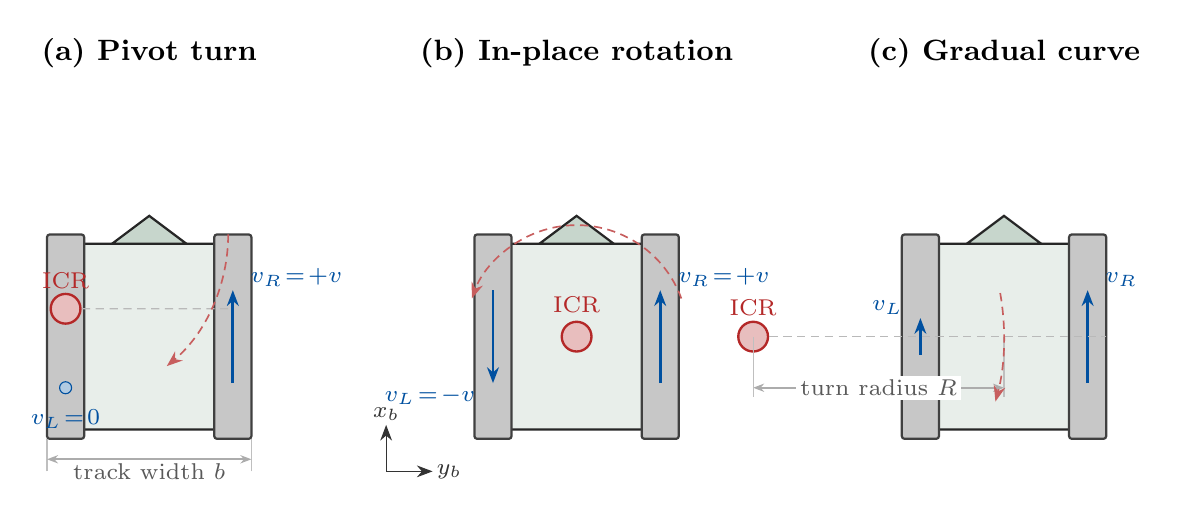
\begin{tikzpicture}[
    scale=1.18, every node/.style={transform shape},
    font=\small,
    >={Stealth[length=2.0mm, width=1.5mm]},
    track/.style={draw=black!75, thick, fill=black!22, rounded corners=1pt},
    body/.style={draw=black!85, thick, fill=cppgreen!10, rounded corners=2.5pt},
    nose/.style={draw=black!85, thick, fill=cppgreen!25}, % small heading triangle
    vel/.style={->, line width=1.0pt, codeblue},
    velzero/.style={draw=codeblue, fill=codeblue!30, circle, inner sep=1.3pt},
    icr/.style={circle, draw=warnred, line width=0.85pt, fill=warnred!30, minimum size=0.32cm, inner sep=0pt},
    icrlabel/.style={font=\scriptsize, warnred, inner sep=1pt},
    radlabel/.style={font=\scriptsize, gray!70!black, fill=white, inner sep=1.2pt},
    velabel/.style={font=\scriptsize, codeblue, inner sep=1pt},
    arc/.style={->, semithick, densely dashed, warnred!75},
    title/.style={font=\small\bfseries},
    dim/.style={<->, gray!65, semithick, >={Stealth[length=1.4mm]}},
    extline/.style={gray!50, thin},
    dimtxt/.style={font=\scriptsize, gray!70!black},
    radline/.style={gray!55, thin, densely dashed},
]

% =========================================================================
% Panel (a): PIVOT TURN     v_L = 0,  v_R = +v
% =========================================================================
\begin{scope}[shift={(0,0)}]
    \node[title] at (1.0, 3.05) {(a) Pivot turn};

    % body + tracks
    \draw[body] (0.2,-1.0) rectangle (1.8,1.0);
    % heading nose (triangle on top edge to indicate "front")
    \fill[nose] (0.6,1.0) -- (1.0,1.30) -- (1.4,1.0) -- cycle;
    \draw[track] (-0.1,-1.1) rectangle (0.3,1.1);
    \draw[track] (1.7,-1.1) rectangle (2.1,1.1);

    % --- velocity arrows (proportional: reference length 1.0 cm = |v|) ---
    % left track stationary: blue ringed dot (placed BELOW the ICR on the same track)
    \node[velzero] (lz) at (0.1, -0.55) {};
    \node[velabel, anchor=north] at (0.1, -0.75) {$v_L\!=\!0$};
    % right track: +v forward, length = 1.0 — label CLEAR of the arrow tip
    \draw[vel] (1.9, -0.50) -- (1.9, 0.50);
    \node[velabel, anchor=south west, inner sep=1pt] at (2.05, 0.50) {$v_R\!=\!+v$};

    % --- ICR coincident with stopped left track centerpoint ---
    \node[icr] (icr1) at (0.1, 0.30) {};
    \draw[radline] (icr1.east) -- (1.85, 0.30);  % visualizes that ICR is on left-track axis
    \node[icrlabel, anchor=south] at (0.10, 0.48) {$\mathrm{ICR}$};

    % --- rotation arc (CCW about ICR, sweeping from front to right side) ---
    \draw[arc] (1.85, 1.10) arc[start angle=0, end angle=-50, radius=1.85cm];

    % --- track width b dimension ---
    \draw[extline] (-0.1,-1.45) -- (-0.1,-1.10);
    \draw[extline] ( 2.1,-1.45) -- ( 2.1,-1.10);
    \draw[dim]    (-0.1,-1.32) -- ( 2.1,-1.32);
    \node[dimtxt] at (1.0,-1.45) {track width $b$};
\end{scope}

% =========================================================================
% Panel (b): IN-PLACE ROTATION    v_L = -v, v_R = +v
% =========================================================================
\begin{scope}[shift={(4.6,0)}]
    \node[title] at (1.0, 3.05) {(b) In-place rotation};

    \draw[body] (0.2,-1.0) rectangle (1.8,1.0);
    \fill[nose] (0.6,1.0) -- (1.0,1.30) -- (1.4,1.0) -- cycle;
    \draw[track] (-0.1,-1.1) rectangle (0.3,1.1);
    \draw[track] (1.7,-1.1) rectangle (2.1,1.1);

    % --- velocity arrows: equal magnitude, opposite signs (length = 1.0 each) ---
    \draw[vel] (0.1,  0.50) -- (0.1, -0.50);
    \node[velabel, anchor=north east, inner sep=1pt] at (-0.05, -0.50) {$v_L\!=\!-v$};
    \draw[vel] (1.9, -0.50) -- (1.9,  0.50);
    \node[velabel, anchor=south west, inner sep=1pt] at (2.05,  0.50) {$v_R\!=\!+v$};

    % --- ICR at geometric center; label INSIDE the body so it doesn't cross arrows ---
    \node[icr] (icr2) at (1.0, 0.0) {};
    \node[icrlabel, anchor=south] at (1.0, 0.22) {$\mathrm{ICR}$};

    % --- rotation arc (full-ish CCW around ICR) ---
    \draw[arc] (1.0,0) ++(20:1.20) arc[start angle=20, end angle=160, radius=1.20cm];

    % --- body-frame axes (placed once, in panel b) ---
    \begin{scope}[shift={(-1.05,-1.45)}]
        \draw[->, black!80, thin] (0,0) -- (0.50,0) node[font=\scriptsize, anchor=west, inner sep=1pt]{$y_b$};
        \draw[->, black!80, thin] (0,0) -- (0,0.50) node[font=\scriptsize, anchor=south, inner sep=1pt]{$x_b$};
    \end{scope}
\end{scope}

% =========================================================================
% Panel (c): GRADUAL CURVE    v_L < v_R   (both forward)
% =========================================================================
\begin{scope}[shift={(9.2,0)}]
    \node[title] at (1.0, 3.05) {(c) Gradual curve};

    \draw[body] (0.2,-1.0) rectangle (1.8,1.0);
    \fill[nose] (0.6,1.0) -- (1.0,1.30) -- (1.4,1.0) -- cycle;
    \draw[track] (-0.1,-1.1) rectangle (0.3,1.1);
    \draw[track] (1.7,-1.1) rectangle (2.1,1.1);

    % --- velocity arrows: v_L short (0.40), v_R long (1.00) — proportional ---
    \draw[vel] (0.1, -0.20) -- (0.1,  0.20);
    \node[velabel, anchor=south east, inner sep=1pt] at (-0.05, 0.20) {$v_L$};
    \draw[vel] (1.9, -0.50) -- (1.9,  0.50);
    \node[velabel, anchor=south west, inner sep=1pt] at (2.05, 0.50) {$v_R$};

    % --- ICR to the left of the body on the wheel-axle line (y=0) ---
    \node[icr] (icr3) at (-1.70, 0.0) {};
    \node[icrlabel, anchor=south, inner sep=1pt] at (-1.70, 0.18) {$\mathrm{ICR}$};

    % --- single dashed radius line from ICR to far track edge (no overlap) ---
    \draw[radline] (icr3) -- (2.1, 0.0);

    % --- R dimension: from ICR to body centerline, with tick marks and label ---
    \draw[dim] (-1.70, -0.55) -- (1.0, -0.55);
    \draw[extline] (-1.70, 0.0) -- (-1.70, -0.65);
    \draw[extline] (1.0,   0.0) -- (1.0,   -0.65);
    \node[dimtxt, fill=white, inner sep=1.2pt] at (-0.35, -0.55) {turn radius $R$};

    % --- arc segment indicating the swept curve path ---
    \draw[arc] (icr3) ++(10:2.70) arc[start angle=10, end angle=-15, radius=2.70cm];
\end{scope}

\end{tikzpicture}

    \caption{Three differential-drive operating modes commanded through a single
    $(v,\omega)$ target. Blue arrows show each track's linear velocity, with
    arrow length proportional to $|v|$; the red ringed marker is the
    instantaneous center of rotation ($\mathrm{ICR}$). Track width $b$ is
    dimensioned once in panel (a) and is identical for all three panels.}
    \label{fig:diff_drive_kinematics}
\end{figure}

The full electromechanical signal path is shown in Figure~\ref{fig:drivetrain_block}.
The Jetson Orin issues \texttt{geometry\_msgs/}\allowbreak\texttt{Twist} commands at
50~Hz to a Teensy~4.1 motion bridge, which decomposes them into per-side wheel
velocities and forwards them over CAN at 1~Mbit/s to the two SparkMAX controllers.
Each SparkMAX closes a velocity loop around its NEO motor at 1~kHz using the integrated
Hall encoders.

\begin{figure}[H]
    \centering
    % Drivetrain signal chain: Jetson -> Teensy -> 2x SparkMAX (CAN) -> 2x NEO -> tracks
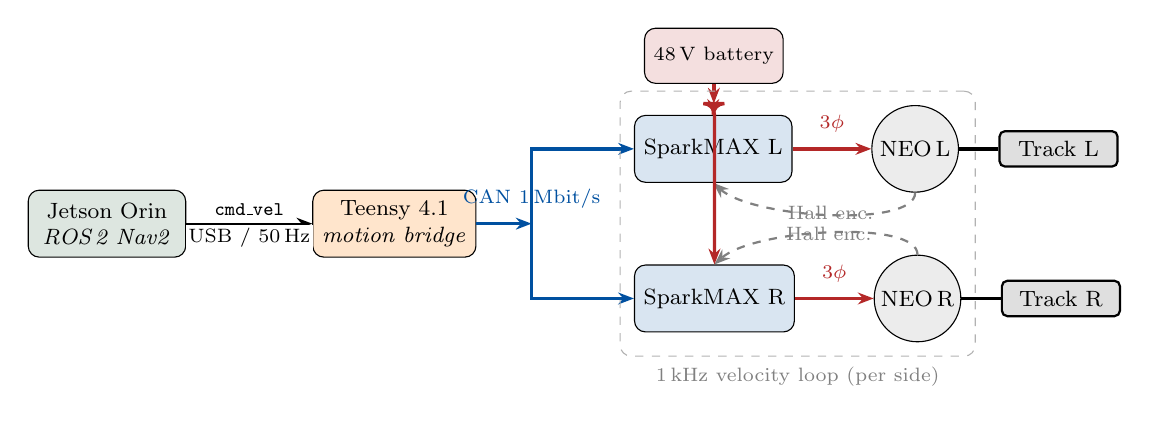
\begin{tikzpicture}[
    font=\footnotesize,
    compute/.style={draw, rounded corners, fill=cppgreen!15, minimum width=2.0cm, minimum height=0.85cm, align=center},
    mcu/.style={draw, rounded corners, fill=orange!20, minimum width=2.0cm, minimum height=0.85cm, align=center},
    drv/.style={draw, rounded corners, fill=codeblue!15, minimum width=2.0cm, minimum height=0.85cm, align=center},
    motor/.style={draw, circle, fill=gray!15, minimum size=1.1cm, align=center, inner sep=1pt},
    track/.style={draw, thick, fill=gray!25, minimum width=1.5cm, minimum height=0.45cm, align=center, rounded corners=2pt},
    batt/.style={draw, rounded corners, fill=warnred!15, minimum width=1.6cm, minimum height=0.7cm, align=center, font=\scriptsize},
    arr/.style={-{Stealth[length=2mm]}, thick},
    busarr/.style={-{Stealth[length=2mm]}, very thick, codeblue},
    pwr/.style={-{Stealth[length=2mm]}, very thick, warnred},
    lbl/.style={font=\scriptsize, midway, above, sloped},
    plbl/.style={font=\scriptsize, midway, above},
    grp/.style={draw, dashed, rounded corners, gray!60, inner sep=5pt},
]

% --- Compute (left) ---
\node[compute] (jetson) {Jetson Orin\\\textit{ROS\,2 Nav2}};
% --- MCU bridge ---
\node[mcu, right=1.6cm of jetson] (teensy) {Teensy 4.1\\\textit{motion bridge}};

% --- SparkMAX pair (split vertically) ---
\node[drv, right=2.0cm of teensy, yshift=0.95cm] (spkL) {SparkMAX L};
\node[drv, right=2.0cm of teensy, yshift=-0.95cm] (spkR) {SparkMAX R};

% --- NEO motors ---
\node[motor, right=1.0cm of spkL] (neoL) {NEO\,L};
\node[motor, right=1.0cm of spkR] (neoR) {NEO\,R};

% --- Tracks ---
\node[track, right=0.5cm of neoL] (trkL) {Track L};
\node[track, right=0.5cm of neoR] (trkR) {Track R};

% --- Battery (placed above, feeding both SparkMAX with single arrow) ---
\coordinate (sparkmid) at ($(spkL.north)!0.5!(spkR.north)$);
\node[batt] (batt) at ($(sparkmid)+(0,1.7)$) {48\,V battery};

% --- Signal: Jetson -> Teensy (USB serial) ---
\draw[arr] (jetson) -- (teensy);
\node[font=\scriptsize, fill=white, inner sep=1pt] at ($(jetson.east)!0.5!(teensy.west)+(0,0.18)$) {\texttt{cmd\_vel}};
\node[font=\scriptsize, fill=white, inner sep=1pt] at ($(jetson.east)!0.5!(teensy.west)+(0,-0.18)$) {USB / 50\,Hz};

% --- Teensy -> CAN bus -> two SparkMAX ---
\coordinate (canjct) at ($(teensy.east)+(0.7,0)$);
\draw[busarr] (teensy.east) -- (canjct);
\node[font=\scriptsize, codeblue, above=2pt of canjct] {CAN 1\,Mbit/s};
\draw[busarr] (canjct) |- (spkL.west);
\draw[busarr] (canjct) |- (spkR.west);

% --- SparkMAX -> NEO (3-phase power) ---
\draw[pwr] (spkL.east) -- (neoL.west);
\node[font=\scriptsize, warnred, above=1pt] at ($(spkL.east)!0.5!(neoL.west)+(0,0.05)$) {3$\phi$};
\draw[pwr] (spkR.east) -- (neoR.west);
\node[font=\scriptsize, warnred, above=1pt] at ($(spkR.east)!0.5!(neoR.west)+(0,0.05)$) {3$\phi$};

% --- NEO -> track (mechanical) ---
\draw[line width=1.2pt] (neoL.east) -- (trkL.west);
\draw[line width=1.2pt] (neoR.east) -- (trkR.west);

% --- Encoder feedback loops (NEO -> SparkMAX, dashed) ---
\draw[arr, dashed, gray] (neoL.south) .. controls +(0,-0.45) and +(0.5,-0.45) .. (spkL.south)
    node[midway, below=1pt, font=\scriptsize, gray]{Hall enc.};
\draw[arr, dashed, gray] (neoR.north) .. controls +(0,0.45) and +(0.5,0.45) .. (spkR.north)
    node[midway, above=1pt, font=\scriptsize, gray]{Hall enc.};

% --- 48V supply: one arrow splits down to both SparkMAX ---
\coordinate (battfan) at ($(batt.south)+(0,-0.25)$);
\draw[pwr] (batt.south) -- (battfan);
\draw[pwr, rounded corners=4pt] (battfan) -| (spkL.north);
\draw[pwr, rounded corners=4pt] (battfan) -| (spkR.north);

% --- Group indicating closed-loop velocity control ---
\node[grp, fit=(spkL)(spkR)(neoL)(neoR),
      label={[font=\scriptsize, gray, anchor=north]below:1\,kHz velocity loop (per side)}] {};

\end{tikzpicture}

    \caption{Drivetrain signal chain. The Jetson plans at 50~Hz; the Teensy converts
    Twist commands to per-side wheel velocities and bridges USB$\rightarrow$CAN; each
    SparkMAX closes a 1~kHz velocity loop around its NEO motor.}
    \label{fig:drivetrain_block}
\end{figure}

\subsection{Weatherproofing}

Outdoor operation requires the electronics bay to tolerate rain and direct sun. The
sensor-shelf walls are formed from cut-to-fit acrylic panels that slide directly into the
20-Series T-slot grooves; weatherstripping gasket fills the residual gap and remains
seated under the vibration produced by the tracks. The top panel is mildly angled so
that water runs off rather than pools, and incorporates a sliding access door for
servicing wiring, replacing the payload, or accessing the compute. The LiDAR is mounted
externally above the shelf to keep its $360^\circ$ field of view unobstructed; the ZED~X
cameras sit behind their own AR-coated windows in the front-facing acrylic.

\subsection{Constraints and Compliance}

IGVC requires a minimum vehicle length of 3~ft and an E-stop mounted between 2~ft and
4~ft above the ground, centered on the rear. To meet both, the original chassis was
extended with a rear-mounted shelf that carries the mechanical E-stop button at $24''$
height (Figure~\ref{fig:cad_rear}). The extension also creates space for the
counter-balanced battery placement without forcing the payload bay forward of the
tracks, where it would adversely shift the CoG.

\subsection{Safety}

The safety architecture (Figure~\ref{fig:safety_block}) implements a hardware-enforced
two-channel emergency stop: either the rear-mounted mechanical E-stop button or the
wireless remote E-stop receiver opens a relay in series with the motor-controller
enable line. When the relay opens the SparkMAX controllers immediately disable PWM
output and brake the NEO motors via the integrated short-brake mode; software is not in
the loop, so a Jetson hang or ROS crash cannot defeat the stop. Indicator LEDs visible
from outside the chassis show the armed/disarmed state for the IGVC safety inspection.

\begin{figure}[H]
    \centering
    % Two-channel E-stop hardware schematic: mechanical button + wireless receiver
% feeding a series enable line into the SparkMAX motor controllers.
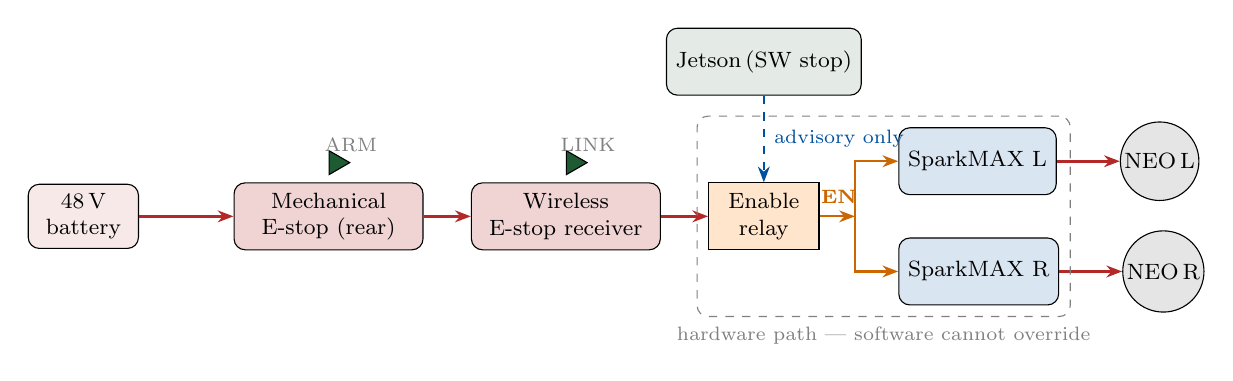
\begin{tikzpicture}[
    font=\footnotesize,
    src/.style={draw, rounded corners, fill=warnred!20, minimum width=2.4cm, minimum height=0.85cm, align=center},
    relay/.style={draw, fill=orange!20, minimum width=1.4cm, minimum height=0.85cm, align=center},
    ctrl/.style={draw, rounded corners, fill=codeblue!15, minimum width=2.0cm, minimum height=0.85cm, align=center},
    motor/.style={draw, circle, fill=gray!20, minimum size=0.95cm, inner sep=1pt},
    batt/.style={draw, rounded corners, fill=warnred!10, minimum width=1.4cm, minimum height=0.7cm, align=center},
    pwr/.style={-{Stealth[length=2mm]}, very thick, warnred},
    sig/.style={-{Stealth[length=2mm]}, thick, codeblue},
    en/.style={-{Stealth[length=2mm]}, thick, orange!80!black},
    led/.style={draw, fill=cppgreen, regular polygon, regular polygon sides=3, minimum size=0.35cm, inner sep=0pt, rotate=-90},
    note/.style={font=\scriptsize, gray, align=center},
]

% --- Power source ---
\node[batt] (batt) at (0,0) {48\,V\\battery};

% --- Two E-stop channels in series along the enable line ---
\node[src, right=1.2cm of batt] (mech) {Mechanical\\E-stop (rear)};
\node[src, right=0.6cm of mech] (wless) {Wireless\\E-stop receiver};

% --- Series relay ---
\node[relay, right=0.6cm of wless] (relay) {Enable\\relay};

% --- Motor controllers ---
\node[ctrl, right=1.0cm of relay, yshift=0.7cm] (spkL) {SparkMAX L};
\node[ctrl, right=1.0cm of relay, yshift=-0.7cm] (spkR) {SparkMAX R};

% --- Motors ---
\node[motor, right=0.8cm of spkL] (neoL) {NEO\,L};
\node[motor, right=0.8cm of spkR] (neoR) {NEO\,R};

% --- Power rail (red) ---
\draw[pwr] (batt.east) -- (mech.west);
\draw[pwr] (mech.east) -- (wless.west);
\draw[pwr] (wless.east) -- (relay.west);

% --- Enable distributed to both SparkMAX ---
\coordinate (jct) at ($(relay.east)+(0.45,0)$);
\draw[en] (relay.east) -- (jct);
\draw[en] (jct) |- (spkL.west);
\draw[en] (jct) |- (spkR.west);
\node[font=\scriptsize\bfseries, orange!80!black, above=1pt] at ($(relay.east)!0.55!(jct)$) {EN};

% --- 3-phase out to motors ---
\draw[pwr] (spkL.east) -- (neoL.west);
\draw[pwr] (spkR.east) -- (neoR.west);

% --- Indicator LEDs (external visibility) ---
\node[led, above=0.25cm of mech] (led1) {};
\node[note, above=0.02cm of led1] {ARM};
\node[led, above=0.25cm of wless] (led2) {};
\node[note, above=0.02cm of led2] {LINK};

% --- Software bypass annotation (negative) ---
\node[draw, dashed, gray, rounded corners, fit=(relay)(spkL)(spkR), inner sep=4pt, label={[font=\scriptsize, gray, anchor=north]below:hardware path --- software cannot override}] {};

% --- Optional Jetson "soft stop" channel (informational, dashed) ---
\node[ctrl, fill=cppgreen!12, above=1.1cm of relay] (jetson) {Jetson\,(SW stop)};
\draw[sig, dashed] (jetson.south) -- (relay.north)
    node[midway, right, font=\scriptsize]{advisory only};

\end{tikzpicture}

    \caption{Two-channel emergency stop. The mechanical (rear-shelf) and wireless E-stops
    are wired in series with the motor-enable relay; either one open de-energizes both
    SparkMAX controllers, independent of software state.}
    \label{fig:safety_block}
\end{figure}

% ----- References -----
\subsection*{References (Mechanical)}
\small
\sloppy
\begin{enumerate}[label={[\arabic*]}]
    \item AndyMark Inc., \textit{Raptor Track Drive}, product page,
    \url{https://andymark.com/products/raptor-track-drive}.
    \item 80/20 Inc., \textit{20-Series T-Slot Aluminum Framing}, product catalog,
    \url{https://8020.net/}.
    \item REV Robotics, \textit{NEO Brushless Motor and SPARK~MAX Motor Controller User
    Manuals}, \url{https://www.revrobotics.com/}.
    \item IGVC, \textit{IGVC 2026 Rules and Course Requirements}, Section 4 (vehicle
    configuration), \url{http://www.igvc.org/}.
\end{enumerate}

\end{document}
